% Glossar
%\setglossarysection{section}
%\glsaddall
\setglossarysection{chapter}
\printglossary[numberedsection,style=altlist,title=Begriffsdefinitionen]
\label{chap:Definitionen}

\chapter{Anforderungsermittlung}


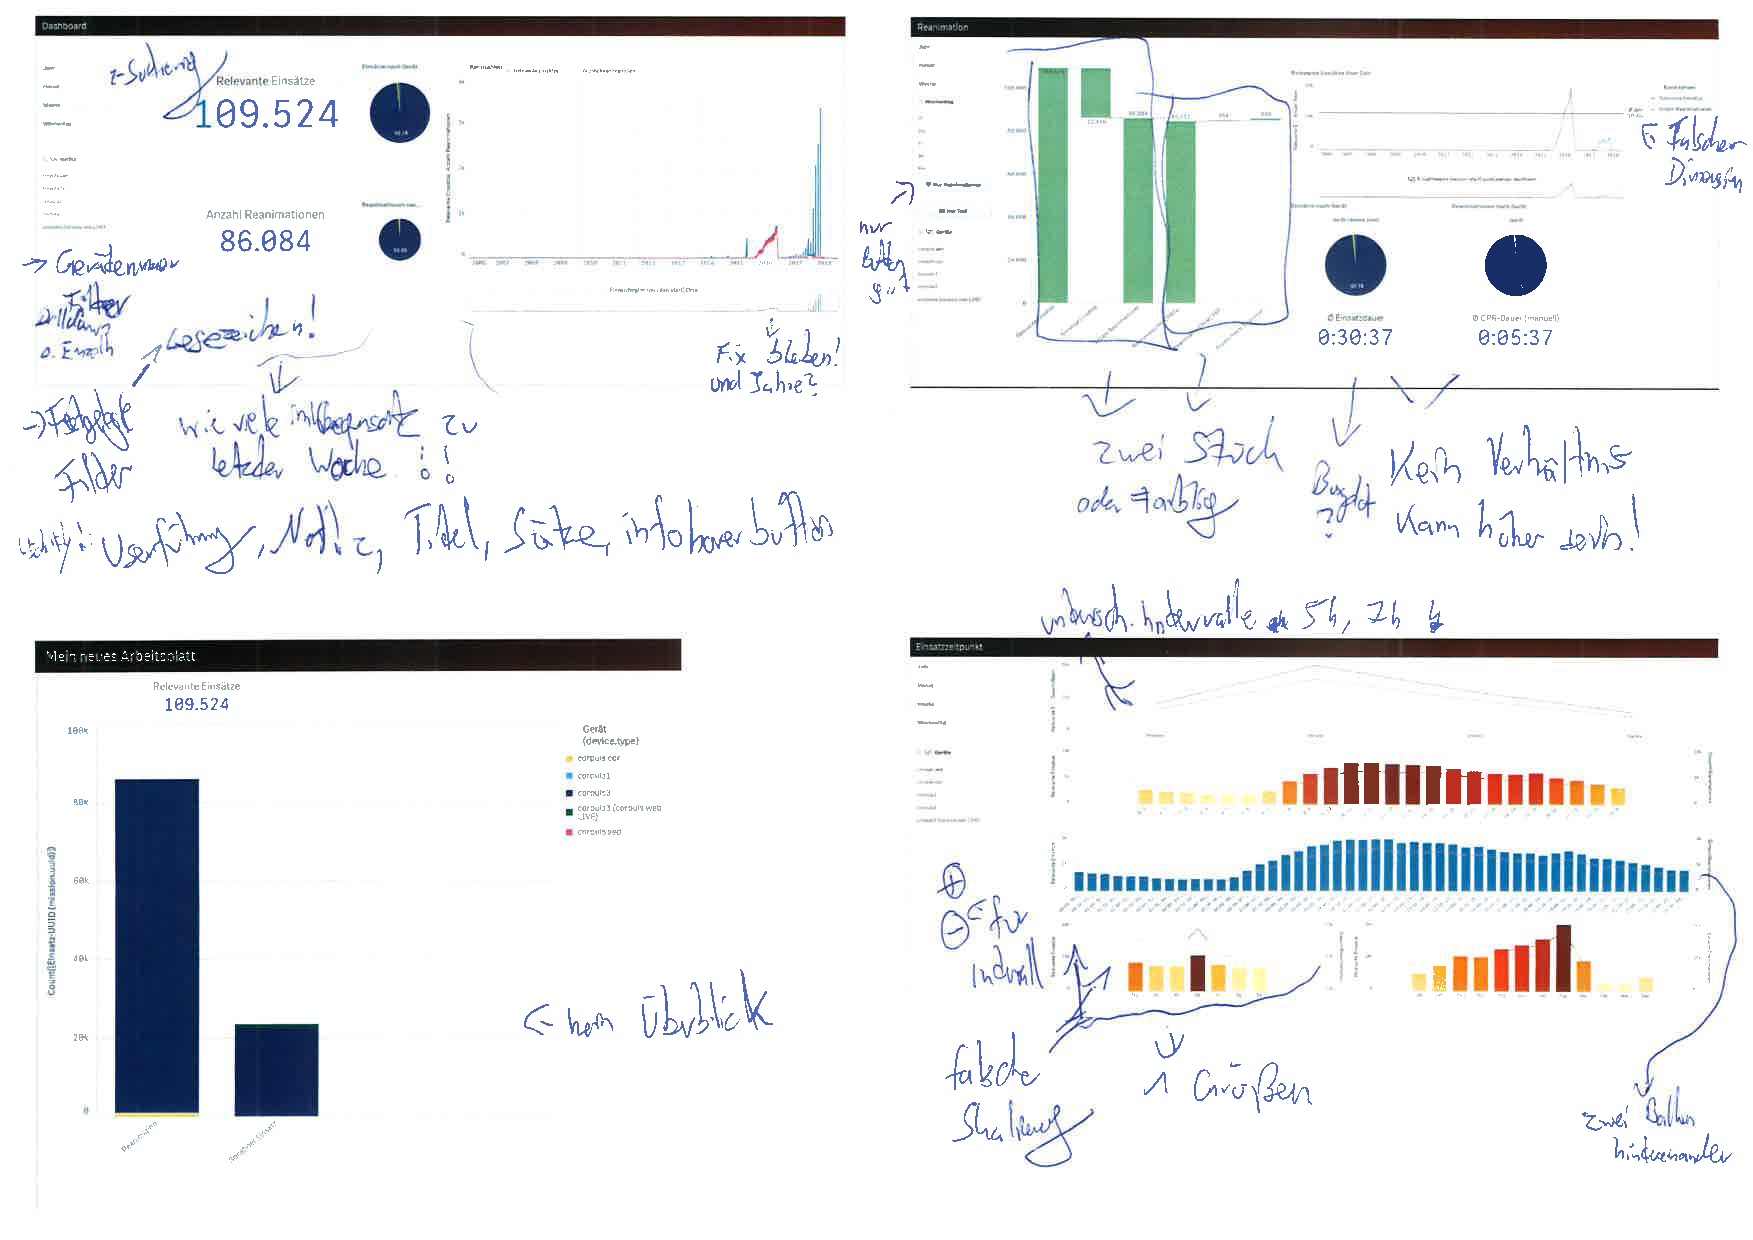
\includepdf[pages=1-2, nup=1x2, scale=0.7, pagecommand=\chapter{Evaluation}\label{att:evaluation}, offset=0 -2cm]{attachments/ALL_EVALUATION2.pdf}
%\includepdf[pages=3, nup=1x2, scale=0.7]{attachments/ALL_EVALUATION2.pdf}
\includepdf[pages=4-15, nup=2x2, scale=0.8,  pagecommand=\thispagestyle{headings}]{attachments/ALL_EVALUATION2.pdf}
\includepdf[pages={3, 16-22}, nup=1x2, scale=0.8, pagecommand=\thispagestyle{headings}]{attachments/ALL_EVALUATION2.pdf}

%\chapter{Dashboards}
%\includepdf[pages=-, nup=1x2, scale=0.6, landscape=true]{attachments/d12.pdf}

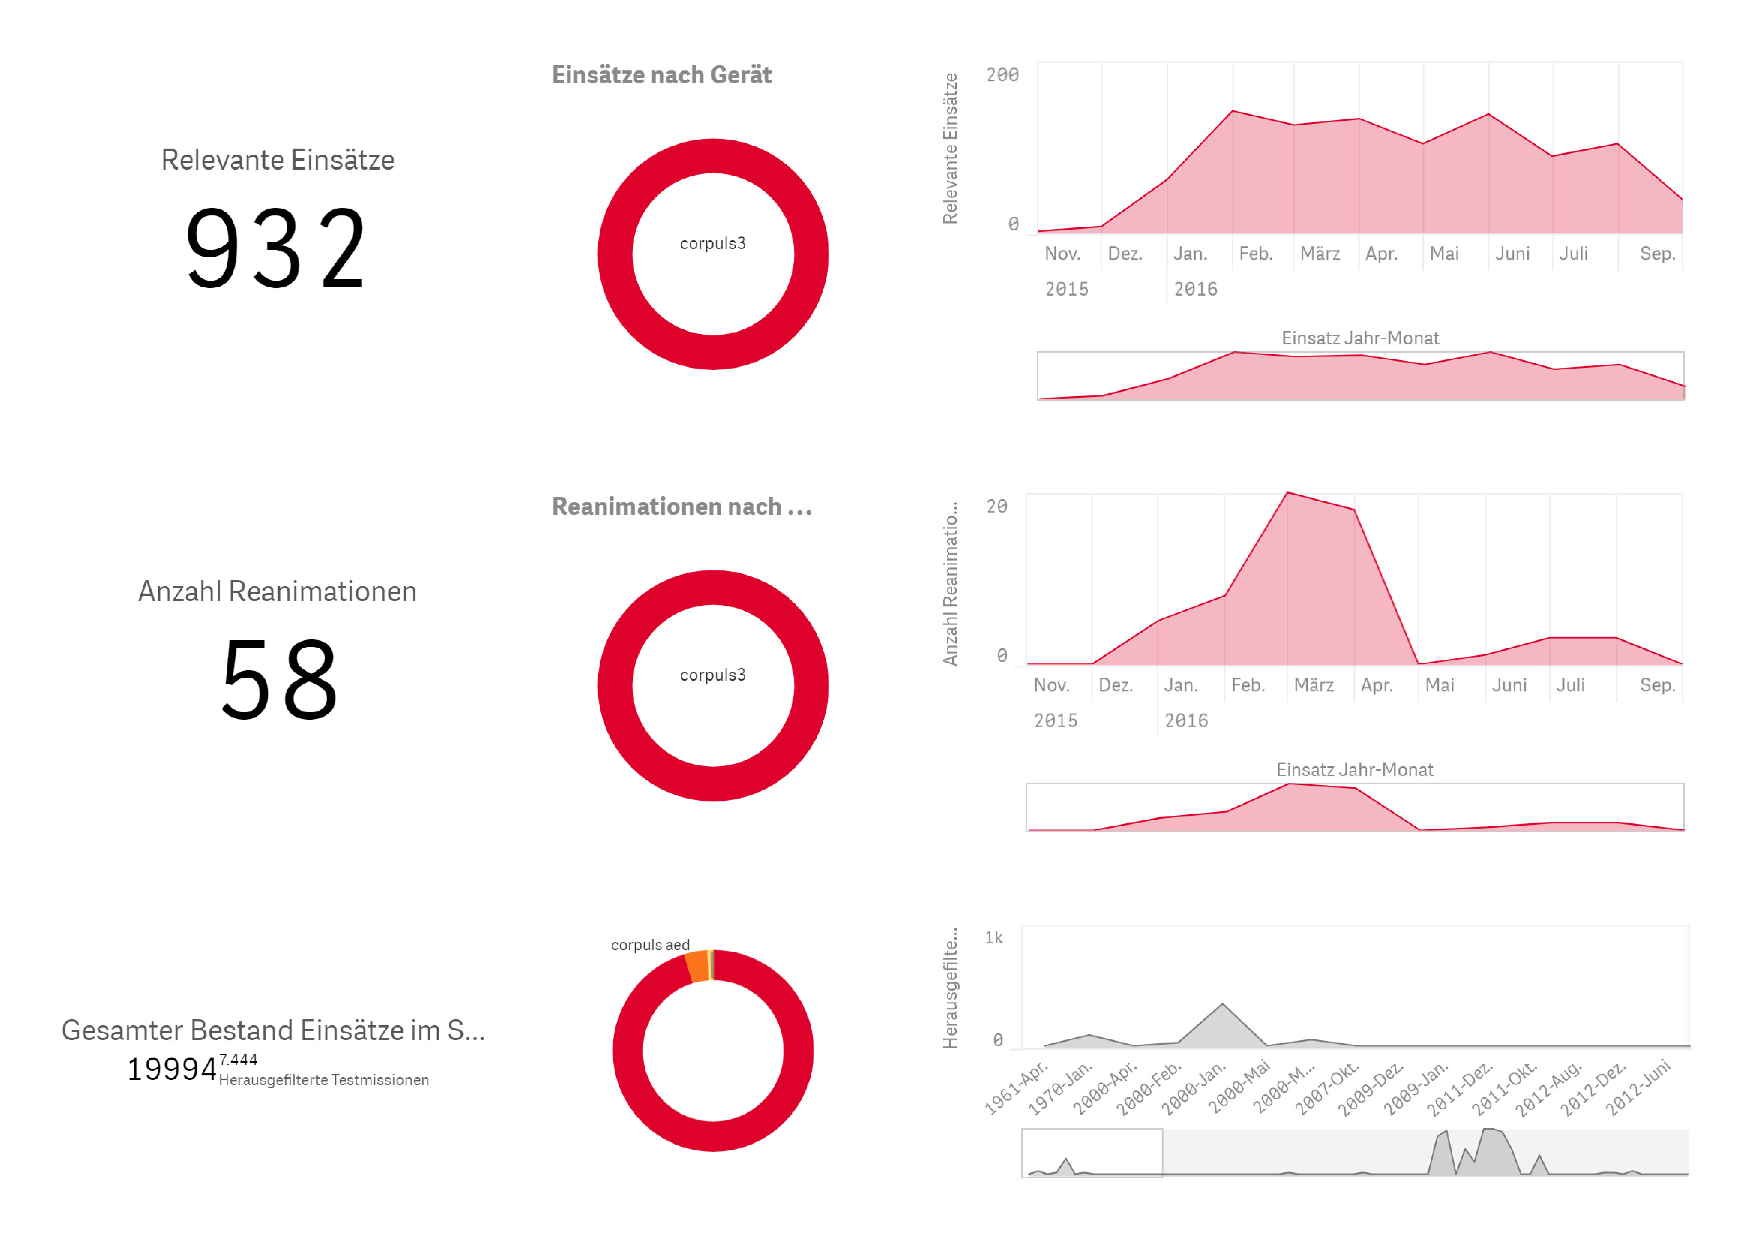
\includepdf[pages=-, nup=1x2, scale=0.7, pagecommand=\chapter{Dashboards}\label{att:dashboards}, offset=0 -2cm]{attachments/d12A1b.pdf}

\chapter{JSON Custom Theme}
